\documentclass{article}
\usepackage{tikz}
\usepackage{amsmath}

\begin{document}

\section*{Consistent Node Ordering for FEM Elements}

\subsection*{Four-Node Isoparametric Quadrilateral Element}

In a four-node isoparametric quadrilateral element, nodes should be oriented in a consistent order, typically counterclockwise starting from the bottom-left corner. The node numbering is as follows:

\[
\text{Node Order: } 1 \rightarrow 2 \rightarrow 3 \rightarrow 4
\]

\begin{center}
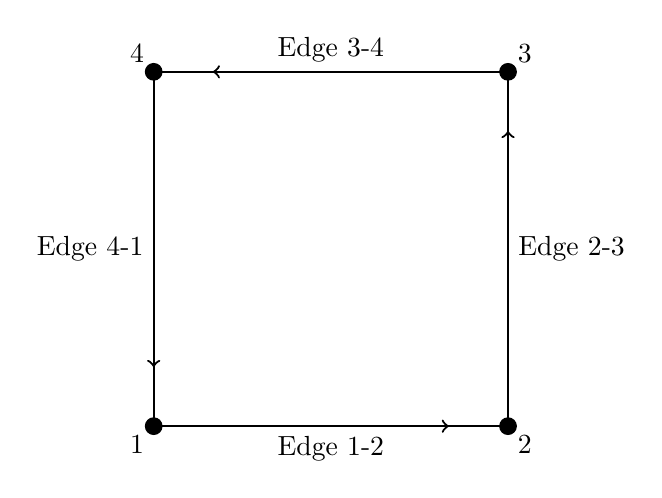
\begin{tikzpicture}[scale=1.5]
    % Draw the quadrilateral
    \draw[thick] (0, 0) -- (3, 0) -- (3, 3) -- (0, 3) -- cycle;
    
    % Draw nodes
    \filldraw[black] (0, 0) circle (2pt) node[below left] {1};
    \filldraw[black] (3, 0) circle (2pt) node[below right] {2};
    \filldraw[black] (3, 3) circle (2pt) node[above right] {3};
    \filldraw[black] (0, 3) circle (2pt) node[above left] {4};

    % Add arrows for counterclockwise orientation
    \draw[->, thick] (0.5, 0) -- (2.5, 0) node[midway, below] {Edge 1-2};
    \draw[->, thick] (3, 0.5) -- (3, 2.5) node[midway, right] {Edge 2-3};
    \draw[->, thick] (2.5, 3) -- (0.5, 3) node[midway, above] {Edge 3-4};
    \draw[->, thick] (0, 2.5) -- (0, 0.5) node[midway, left] {Edge 4-1};
\end{tikzpicture}
\end{center}

\subsection*{Jacobian Determinant for Orientation Check}

The Jacobian determinant \( \det(J) \) is used to verify the orientation of elements. For a correctly oriented element (counterclockwise), \( \det(J) > 0 \). For a flipped element (clockwise), \( \det(J) < 0 \).

To check the orientation:
\[
\det(J) = \frac{\partial x}{\partial \xi} \frac{\partial y}{\partial \eta} - \frac{\partial x}{\partial \eta} \frac{\partial y}{\partial \xi}
\]

\subsection*{Example of Incorrect Orientation (Flipped Element)}

If nodes are ordered clockwise (e.g., \( 1 \rightarrow 4 \rightarrow 3 \rightarrow 2 \)), the element is flipped:

\begin{center}
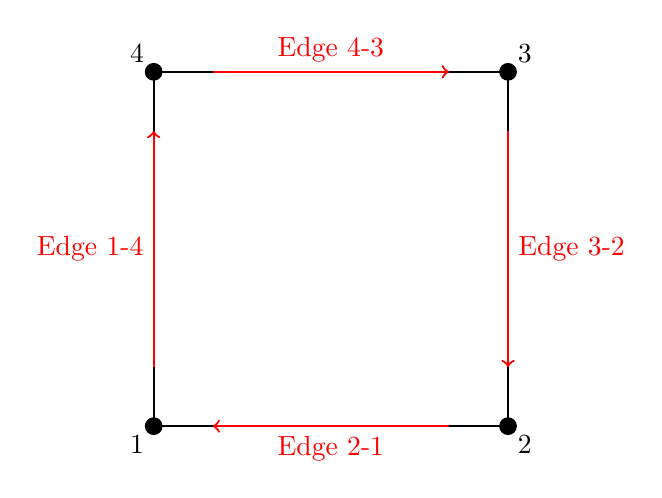
\begin{tikzpicture}[scale=1.5]
    % Draw the quadrilateral
    \draw[thick] (0, 0) -- (0, 3) -- (3, 3) -- (3, 0) -- cycle;
    
    % Draw nodes
    \filldraw[black] (0, 0) circle (2pt) node[below left] {1};
    \filldraw[black] (0, 3) circle (2pt) node[above left] {4};
    \filldraw[black] (3, 3) circle (2pt) node[above right] {3};
    \filldraw[black] (3, 0) circle (2pt) node[below right] {2};

    % Add arrows for clockwise orientation
    \draw[->, thick, red] (0, 0.5) -- (0, 2.5) node[midway, left] {Edge 1-4};
    \draw[->, thick, red] (0.5, 3) -- (2.5, 3) node[midway, above] {Edge 4-3};
    \draw[->, thick, red] (3, 2.5) -- (3, 0.5) node[midway, right] {Edge 3-2};
    \draw[->, thick, red] (2.5, 0) -- (0.5, 0) node[midway, below] {Edge 2-1};
\end{tikzpicture}
\end{center}

\textbf{Correct this orientation by reordering nodes to follow a counterclockwise sequence.}

\end{document}
